\section{Reliable Error Estimation Via Cones}\label{SectCones}

\subsection{The Flaws in {\tt integral.m} and Other Automatic, Adaptive Algorithms} \label{drugssubsect} Computations are prevalent in research, development and operations.  These computations solve large complex problems by assembling basic numerical algorithms for sub-problems. Errors in one piece can propagate throughout.  Our focus is on some of these basic algorithms for function approximation and integration.  As explained at the beginning of the proposal, we want these algorithms to be automatic, adaptive, guaranteed, efficient, and stable.

\Matlab's {\tt integral.m} \citep{MAT8.2} is a typical automatic, adaptive quadrature algorithm.  According to its documentation ``{\tt integral} attempts to satisfy {\tt |Q - I| <= max(AbsTol, RelTol*|Q|)}, where {\tt I} denotes the exact value of the integral.'' Although {\tt integral.m} is automatic, adaptive and stable, it has no guarantees of success and no known bound on its computational cost. Automatic quadrature algorithms in other common software packages suffer the same flaws.  We have developed an alternative to {\tt integral.m}, described in Sect.\ \ref{integral_g_sec}, which satisfies all of our desired criteria for reliability and practicality.

\Matlab's {\tt integral.m} begins by splitting the integration interval into ten sub-intervals and applies Gauss-Kronrod quadrature using $15$ nodes on each sub-interval.  The absolute error on a sub-interval is estimated in terms of the difference between two Gauss quadrature rules using the same nodes, $\bigl \lvert Q(f)-\tQ(f) \bigr \rvert$. If the estimated error is too large, the sub-interval is further subdivided and the process is repeated.

This kind of error estimation can fail in two ways as depicted in Fig.\ \ref{MatIntegFailFig}. The first way is for the sampling scheme (in this case $150$ initial data sites) to miss significant \emph{spikes} in the integrand.  Any quadrature scheme is susceptible to this problem, but {\tt integral.m} fails to quantify how spiky integrands can be and still be integrated correctly.

\begin{figure}[h]
\centering
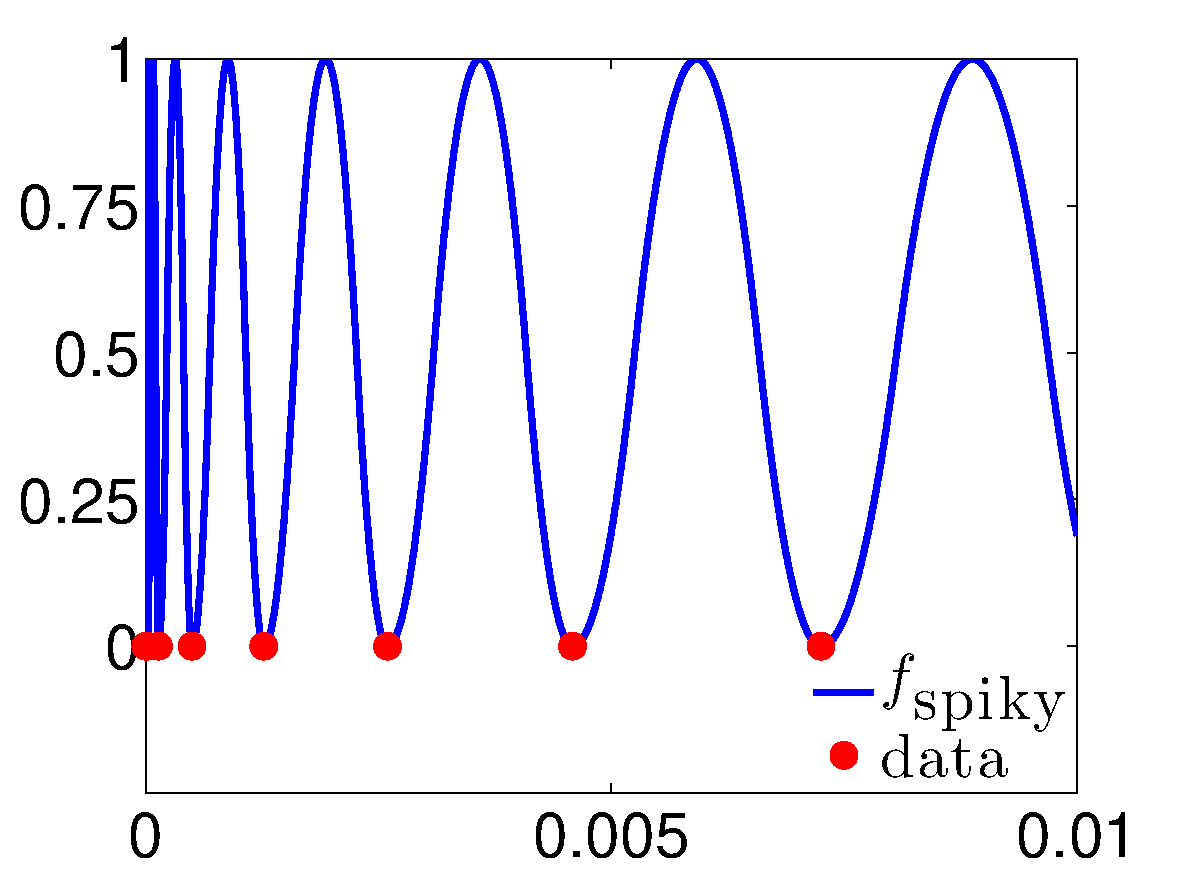
\includegraphics[width=6cm]{SpikyFoolIntegral.eps} \qquad
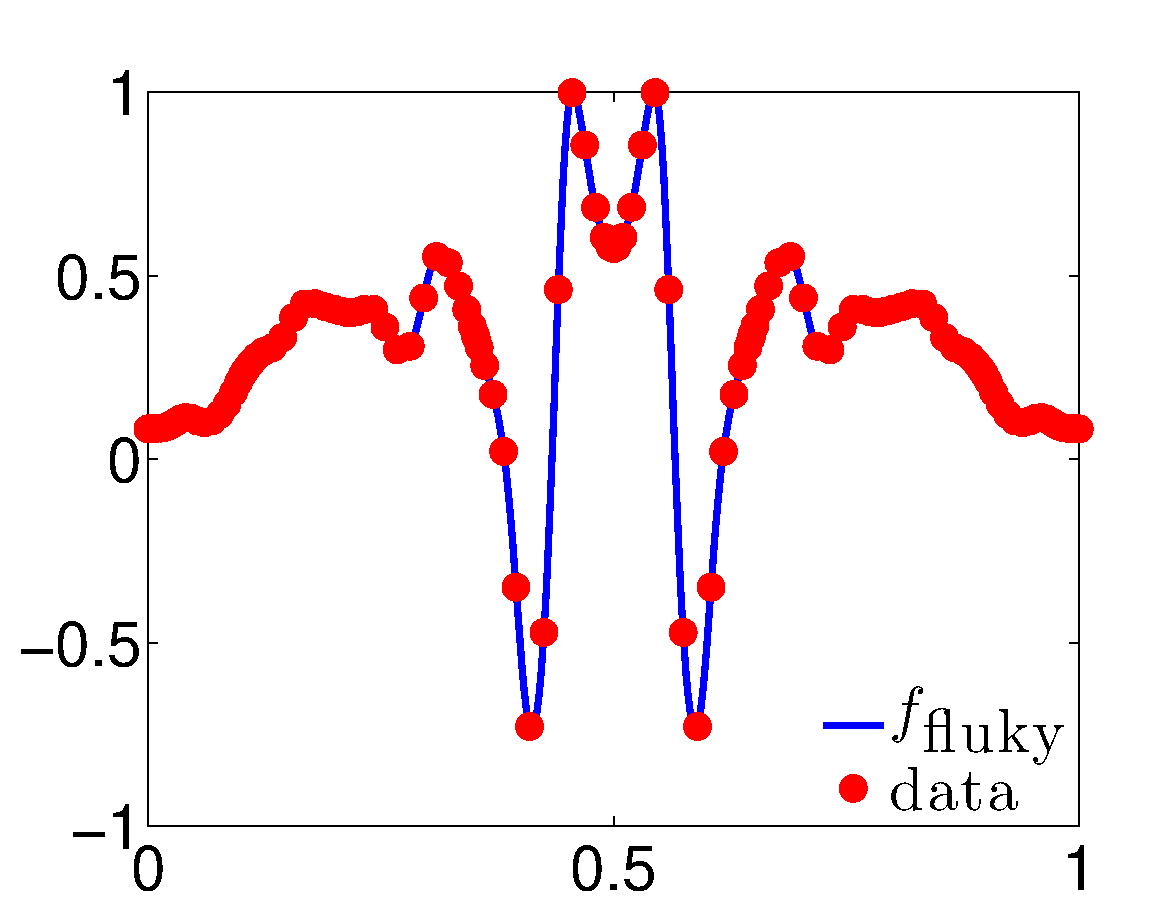
\includegraphics[width=6cm]{FlukyFoolIntegral.eps} \\
$\int_0^1 f_{\text{spiky}}(x) \, \dif x=0.5$, \qquad \qquad $\int_0^1 f_{\text{fluky}}(x) \, \dif x=0.278827$ \\
{\tt integral(fspiky,0,1,'AbsTol',1e-13,'RelTol',1e-13)=0} \\
{\tt integral(ffluky,0,1,'AbsTol',1e-13,'RelTol',1e-13)=0.278799}
\caption{Integrands for which {\tt integral.m} fails to give the answer to within the user-specified tolerance. \label{MatIntegFailFig}}
\end{figure}

The fluctuations of the \emph{fluky} integrand in Fig.\ \ref{MatIntegFailFig} are observed by the sampling scheme, but the error estimate, $\bigl \lvert Q(f)-\tQ(f) \bigr \rvert$, just happens to vanish on each sub-interval. Again, {\tt integral.m} fails to say when this might happen. Thirty years ago, \cite{Lyn83} warned that the error estimates of the form $\bigl \lvert Q(f)-\tQ(f) \bigr \rvert$---used by virtually all automatic quadrature rules---were flawed because they could be fooled by fluky integrands.  Lyness offered no alternative.  \emph{We have one.}

\subsection{Guaranteed Automatic Quadrature via {\tt integral\_g.m}} \label{integral_g_sec} Our guaranteed automatic algorithm for evaluating $\int_0^1 f(x) \, \dif x$ is based on the trapezoidal rule with $n$ trapezoids ($N=n+1$ data) and its well-known error bound \cite[(7.15)]{BraPet11a}:
\begin{equation} \label{traprule}
T_n(f) = \frac{1}{n} \left[f(0) + 2 f\left(\frac 1n \right) + \cdots + 2 f\left(\frac {n-1} n \right) + f(1) \right], \ \
\abs{\int_0^1 f(x) \, \dif x - T_n(f)} \le \frac{\norm[1]{f''}}{8 n^2}.
\end{equation}
Like error bound \eqref{rbferrbd}, this error bound by itself is insufficient for constructing an automatic, adaptive quadrature algorithm because $\norm[1]{f''}$ is unknown in advance.

Our approach assumes that the integrand lies in the cone of functions \citep{HicEtal14b}
\begin{equation} \label{integralcone}
\cc_{n^*} := \{f : \norm[1]{f''} \le 2 n^* \norm[1]{f'-f(1)+f(0)} \},
\end{equation}
namely functions whose stronger semi-norm is bounded in terms of a weaker semi-norm.  We then approximate the weaker norm by replacing $f$ by it linear spline, $S_n(f)$.  Because $\norm[1]{f'}-\norm[1]{S_n(f)'} \le \norm[1]{f''}/(2n)$, we can derive this data-driven upper bound on the error of the trapezoidal rule:
\begin{equation} \label{traperrupbd}
\abs{\int_0^1 f(x) \, \dif x - T_n(f)} \le  \frac{\norm[1]{f''}}{8 n^2} \le \frac{n^* \norm[1]{S_n(f)'-f(1)+f(0)}}{4 n(n - n^*)}, \qquad n>n^*.
\end{equation}

Algorithm 4 in \cite{HicEtal14b} increases $n$ until the right hand side of \eqref{traperrupbd} is no greater than the error tolerance, $\varepsilon$.  This algorithm has been implemented as {\tt integral\_g.m} in the Guaranteed Automatic Integration Library (GAIL) \citep{ChoiEtal13a}.  Like \Matlab's {\tt integral.m}, algorithm {\tt integral\_g.m} is automatic, adaptive, and numerically stable.  However, {\tt integral\_g.m} also satisfies the other required criteria stated at the beginning of the proposal \citep{HicEtal14b}.
\begin{description}[leftmargin=2.5ex]
\item[Guarantee] $\displaystyle \abs{\int_0^1 f(x) \dif x - T_n(f)} \le \varepsilon$ for all $f \in \cc_{n^*}$.
\item[Computational Cost Upper Bound] The number of trapezoids needed does not exceed $\displaystyle 3+2n^*+\sqrt{\frac{n^* \norm[1]{f''}}{2 \varepsilon}}$, where $\norm[1]{f''}$ is not known a priori but bounded by the algorithm using data.
\item[Complexity Lower Bound] Any algorithm that succeeds for all $f \in \cc_{n^*}$ must use at least $\displaystyle -1 + \sqrt{\frac{(n^* - 1) \norm[1]{f''}}{16 n^* \varepsilon}}$ integrand values.  Our {\tt integral\_g.m} has asymptotically optimal computational cost as $\varepsilon/\norm[1]{f''} \to 0$.
\end{description}

The spikiness of the integrands, $f$, for which {\tt integral\_g.m} succeeds is precisely quantified by the condition $f \in \cc_{n^*}$. The parameter $n^*$ has an intuitive interpretation:  the minimum number of trapezoids is $n^*+1$, and $1/n^*$ is the width of the spikes that can barely be observed.  Fluky integrands like the one in Fig.\ \ref{MatIntegFailFig} cannot fool {\tt integral\_g.m} because its error estimation is not based on the difference of two quadrature rules.

Although {\tt integral\_g.m} has the desirable properties listed above, it has \emph{deficiencies that we intend to rectify.}
\begin{itemize}[leftmargin=2.5ex]
\item Our {\tt integral\_g.m} needs to be extended to include a relative error tolerance as well as the present absolute error tolerance.

\item Now {\tt integral\_g.m} is globally adaptive, meaning that the data sites are uniformly spaced, but the number of sites is chosen adaptively.  We need should local adaptivity to improve efficiency for integrands that are spikier in only part of the interval of integration.

\item The trapezoidal rule underlying {\tt integral\_g.m} should be replaced with a higher order rule for greater efficiency.
\end{itemize}

\subsection{Cones Are the Key}
Constructing an automatic, adaptive algorithm that is also \emph{guaranteed}, such as {\tt integral\_g.m}, depends on defining the right cone of input functions.  Adaptive algorithms have no significant advantage over non-adaptive algorithms for problems defined for convex sets of input functions and satisfying certain other reasonable conditions \cite[Chapter 4, Theorem 5.2.1]{TraWasWoz88}. For example, if we want to construct a guaranteed, automatic algorithm for functions in the (convex) ball, $\cb_{\sigma} = \{f : \norm[1]{f''} \le \sigma \}$, then using the trapezoidal rule, $T_n(f)$, with $n=\bigl\lceil\sqrt{\sigma/(8 \varepsilon)}\, \bigr \rceil$ has nearly optimal computational cost, but it is \emph{non-adaptive}.  By requiring integrands to lie inside a non-convex cone, we allow adaption to be useful. We are also able to prove that the algorithm must succeed, bound its computational cost, and bound the computational complexity of the problem.

The arguments leading to {\tt integral\_g.m} are not restricted to univariate integration but have wider possible application \citep{HicEtal14b}.  The main constraint is that the solution operator be positively homogeneous.  \emph{Thus, we plan to develop guaranteed, automatic, adaptive algorithms for other approximation and integration problems as well.}

\subsection{Guaranteed Monte Carlo} \label{MC_g_sec}
\cite{HicEtal14a} have developed {\tt meanMC\_g.m} in GAIL for constructing guaranteed $\varepsilon$-half-width confidence intervals for the mean, $\mu=\bbE(Y)$, of a random variable, $Y$, via independent and identically distributed (IID) Monte Carlo simulation.  We use the sample mean and sample variance:
\begin{equation} \label{samplemean}
\hmu_{N}:=\frac 1{N} \sum_{i=1}^{N} Y_i, \quad \hsigma_{N}^2:=\frac 1{N-1} \sum_{i=1}^N (Y_i-\hmu_{N})^2, \qquad Y_1, Y_2, \ldots \text{ IID}.
\end{equation}
A typical approach is to pick an $n_{\sigma}$, compute $\hsigma_{n_{\sigma}}^2$, perhaps multiply it by an inflation factor $\fC^2>1$ to approximate $\var(Y)=\bbE[(Y-\mu)^2]$, and then appeal to the  Central Limit Theorem (CLT), to construct an approximate confidence interval.  There are no guarantees because the estimate of the variance may be wrong and the CLT is not a finite sample result.

Instead, we assume that $Y$ lies in the \emph{cone} of random variables whose kurtosis, $\bbE[(Y-\mu)^4]/[\var(Y)]^2$, is no greater than a parameter $\kappa_{\max}$, which depends explicitly on $n_{\sigma}$ and $\fC^2$.  The cone condition allows us to use Cantelli's inequality to prove that $\var(Y)\le \fC^2\hsigma_{n_\sigma}^2$ with high probability.  The cone condition also allows us to use a Berry-Esseen inequality to choose $n_{\mu}$ that \emph{guarantees} that $\Pr[\abs{\mu-\hmu_{n_{\mu}}} \le \varepsilon]\le 1-\alpha$, where $\hmu_{n_{\mu}}$ is based on a sample that is independent of the one used to compute $\hsigma_{n_\sigma}^2$.

The multidimensional integral $\int_{\reals^d} f(\bx) \rho(\bx) \, \dif \bx$ can be interpreted as $\mu=\bbE(Y)$ with $Y=f(\bX)$ and $\bX$ having probability density $\rho$. In this way {\tt meanMC\_g.m} can be used for guaranteed automatic, adaptive multidimensional integration (cubature) \citep{HicEtal14a}.  The cone condition $Y$ translates into a cone condition on $f$.

Our {\tt meanMC\_g.m} also lacks the ability to satisfy a relative error tolerance. \emph{We aim to rectify this deficiency.}

\subsection{Other Monte Carlo Research Topics} We intend to develop guaranteed versions of two other versions of Monte Carlo methods:
\begin{description}[leftmargin=2.5ex]
\item[Multi-Level Monte Carlo] In some situations, generating an exact instance of the random variable, $Y$, would take an infinite amount of time, e.g., if $Y$ is an option payoff that depends on the numerical solution of a stochastic differential equation.  Multi-level methods overcome this problem by computing a large number of coarse approximations to $Y$ and a small number of fine approximations to $Y$ (see the PI's work \citep{NiuHic09a, NiuHic09b} and the review by \cite{Gil14a}).  \emph{We will develop guaranteed multi-level Monte Carlo methods.}

\item[Quasi-Monte Carlo] Quasi-Monte Carlo methods \citep{DicEtal14a} reduce the error in approximating $\mu=\bbE(Y)=\int_{\reals^d} f(\bx) \rho(\bx) \, \dif \bx$, by replacing the IID samples, $\bX_1, \bX_2, \ldots$ in $Y_i=f(\bX_i)$ with evenly distributed samples, such as integration lattices or digital nets.  The error can be expressed in terms of the Fourier (complex exponential or Walsh) coefficients of $f$.  We will use the discrete Fourier coefficients of the integrand values, which can be computed in $N \log(N)$ operations, to reliably estimate the error and \emph{construct guaranteed, automatic, adaptive quasi-Monte Carlo cubature algorithms.} The PI has used these fast discrete Fourier transforms in earlier work \citep{LiHic03a,DicHicLiu07a}.

\end{description}

\subsection{Multivariate Function Approximation (Recovery)}\label{SecRecovery}
Constructing reliable and practical  univariate and multivariate integration algorithms as described in the previous subsections are important objectives in their own right.  As relatively easier problems, they also support our \emph{objective of constructing a guaranteed, adaptive, automatic multivariate function approximation algorithm,} as discussed in the introduction.

There exist univariate function approximation algorithms, such as cubic splines, in widely used software packages, but those algorithms are not automatic.  GAIL \citep{ChoiEtal13a} includes a guaranteed, adaptive linear spline algorithm, {\tt funappx\_g.m}, whose theoretical underpinnings resemble those of {\tt integral\_g.m} \citep{HicEtal14b}.  Like {\tt integral\_g.m}, we intend to derive \emph{a higher order version of {\tt funappx\_g.m} that is also locally adaptive and satisfies a relative error tolerance.}

For multivariate function approximation we focus on meshfree approximation \eqref{rbfapprox}.  Here is how we might proceed.  As in Sect.\ \ref{integral_g_sec}, we need to identify a cone of input functions where the stronger norm, i.e., the Hilbert space norm, $\norm[\ch]{\cdot}$, is bounded above by some multiple of a weaker norm.  We might choose the weaker norm to correspond to a Hilbert space, $\tch$, whose reproducing kernel $\tK$ has a Hilbert-Schmidt series involving the same eigenfunctions as $K$ but a more slowly decaying sequence of eigenvalues (see \eqref{HSseries} below). See \eqref{CMatern} and the kernels in \citep[Chap.\ 2]{Wah90} as examples of such kernels.  Analogously to Sect.\ \ref{integral_g_sec}, we would then need to find a bound on $\norm[\tch]{f} - \bigl\lVert \tf \bigr \rVert_{\tch}$ in terms of $\norm[\ch]{f}$ and use the data-driven $\bigl\lVert \tf \bigr \rVert_{\tch}$ to approximate $\norm[\tch]{f}$, which by the cone condition would give an upper bound on $\norm[\ch]{f}$. These calculations would involve the matrices $\mK$ and $\tmK$, which may be ill-conditioned, as mentioned in the introduction.  To make our proposed algorithm numerically stable we need to employ the techniques introduced in the next section.


